% !TEX root = ../main.tex
% File: chapters_part1/chap6_1.tex
% Nội dung cho Chương 6, Phần 1


\section{Tìm kiếm và Sinh Tăng cường (Retrieval-Augmented Generation - RAG)}
\label{sec:rag}

\begin{tcolorbox}[
    title=Trực giác cốt lõi của RAG,
    colback=yellow!10!white, colframe=yellow!50!black, fonttitle=\bfseries
]
Thay vì buộc LLM phải "nhớ" mọi thứ, hãy cho nó làm một "bài kiểm tra mở sách" (open-book exam). Khi nhận được một câu hỏi, thay vì trả lời ngay lập tức từ trí nhớ, hệ thống RAG trước hết sẽ \textbf{tìm kiếm (retrieve)} các thông tin liên quan nhất từ một cơ sở tri thức bên ngoài (ví dụ: tài liệu công ty, Wikipedia, các file PDF). Sau đó, nó sẽ cung cấp các thông tin đã tìm được này, cùng với câu hỏi gốc, cho LLM để \textbf{sinh ra (generate)} một câu trả lời dựa trên các bằng chứng đó.
\end{tcolorbox}

RAG biến LLM từ một "nhà hiền triết" biết tuốt (nhưng đôi khi đãng trí và bịa chuyện) thành một "nhà nghiên cứu" tài ba, có khả năng tìm kiếm, tổng hợp và trả lời dựa trên các nguồn thông tin xác thực.

\subsection{Tại sao và Khi nào chúng ta cần RAG?}
\label{ssec:why_rag}
Trước khi đi sâu vào kỹ thuật, điều quan trọng là phải hiểu rõ các vấn đề mà RAG giải quyết và khi nào nó là công cụ phù hợp.

\paragraph{Các vấn đề cố hữu của LLM}
Các mô hình ngôn ngữ lớn, dù mạnh mẽ đến đâu, vẫn đối mặt với ba thách thức lớn:
\begin{itemize}
    \item \textbf{Bịa đặt thông tin (Hallucination):} LLM có xu hướng tự "sáng tạo" ra các thông tin không có thật một cách rất tự tin, gây ra rủi ro nghiêm trọng trong các ứng dụng đòi hỏi tính chính xác.
    \item \textbf{Giới hạn tri thức (Knowledge Cutoff):} Tri thức của LLM bị đóng băng tại thời điểm nó được huấn luyện. Nó không biết về các sự kiện, dữ liệu hoặc thông tin mới xuất hiện sau ngày đó.
    \item \textbf{Thiếu tính kiểm chứng (Lack of Verifiability):} Khi LLM đưa ra một câu trả lời, rất khó để truy ngược lại nguồn thông tin mà nó đã sử dụng, khiến việc xác thực trở nên bất khả thi.
\end{itemize}
RAG được thiết kế để giải quyết trực tiếp cả ba vấn đề này bằng cách cung cấp cho LLM các bằng chứng cập nhật và có thể kiểm chứng tại thời điểm trả lời.

\paragraph{Khi nào nên sử dụng RAG?}
\begin{itemize}
    \item Khi ứng dụng của bạn cần truy cập vào \textbf{kho tri thức riêng tư, lớn, hoặc thay đổi liên tục} (tài liệu nội bộ, cơ sở dữ liệu sản phẩm, văn bản pháp luật mới). Việc fine-tune lại LLM liên tục là không khả thi và tốn kém.
    \item Khi \textbf{tính chính xác và khả năng trích dẫn nguồn} là yêu cầu bắt buộc (trợ lý pháp lý, tư vấn y tế, tra cứu thông tin tài chính).
    \item Khi mục tiêu chính là \textbf{giảm thiểu rủi ro bịa đặt thông tin} và đảm bảo câu trả lời được neo vào các nguồn xác thực.
\end{itemize}

\subsection{Kiến trúc RAG Cơ bản (The Naive RAG Pipeline)}
\label{ssec:naive_rag}
Một hệ thống RAG cơ bản, thường được gọi là "Naive" hay "Vanilla" RAG, bao gồm hai giai đoạn chính: \textbf{Lập chỉ mục (Indexing)} và \textbf{Truy vấn (Querying)}. Đây là nền tảng để hiểu tất cả các kỹ thuật nâng cao sau này.

\paragraph{Giai đoạn 1: Lập chỉ mục (Offline)}
Giai đoạn này được thực hiện một lần hoặc định kỳ để chuẩn bị cơ sở tri thức. Nó giống như việc chúng ta sắp xếp và tạo mục lục cho một thư viện.
\begin{enumerate}
    \item \textbf{Tải Dữ liệu (Load):} Tải các tài liệu từ nguồn (PDF, TXT, HTML, v.v.).
    \item \textbf{Phân mảnh (Chunk/Split):} Chia các tài liệu dài thành các đoạn nhỏ hơn, gọi là các "chunk". Trong kiến trúc cơ bản, đây thường là \textit{fixed-size chunking} (chia thành các đoạn có kích thước cố định).
    \item \textbf{Nhúng (Embed):} Sử dụng một mô hình nhúng (embedding model, ví dụ: các bi-encoder từ `sentence-transformers`) để chuyển mỗi chunk thành một vector số (embedding). Vector này nắm bắt ngữ nghĩa của chunk đó.
    \item \textbf{Lưu trữ (Store):} Lưu trữ các chunk và các vector embedding tương ứng của chúng vào một \textbf{Cơ sở dữ liệu Vector} (Vector Database) như FAISS, ChromaDB, hoặc pgvector.
\end{enumerate}

\paragraph{Giai đoạn 2: Truy vấn (Online)}
Giai đoạn này xảy ra mỗi khi người dùng đặt câu hỏi.
\begin{enumerate}
    \item \textbf{Nhúng Câu hỏi (Query Embedding):} Câu hỏi của người dùng được nhúng thành một vector truy vấn, sử dụng \textbf{cùng một embedding model} đã dùng ở giai đoạn lập chỉ mục.
    \item \textbf{Tìm kiếm (Retrieve):} Vector truy vấn được sử dụng để thực hiện một \textit{tìm kiếm tương đồng (similarity search)} trong Vector Database, nhằm tìm ra $k$ chunk có vector gần nhất (tương đồng nhất về mặt ngữ nghĩa).
    \item \textbf{Tăng cường Prompt (Augment):} Các chunk đã tìm được được ghép vào prompt cùng với câu hỏi gốc của người dùng.
        \begin{tcolorbox}[colback=gray!5!white, colframe=gray!50!black, sharp corners]
        \textbf{Ngữ cảnh được cung cấp:} \\
        \textit{[Nội dung của chunk 1...]} \\
        \textit{[Nội dung của chunk 2...]} \\
        \textit{[...]} \\
        \textbf{Dựa vào ngữ cảnh trên, hãy trả lời câu hỏi sau:} \\
        \textit{[Câu hỏi gốc của người dùng]} \\
        \textbf{Trả lời:}
        \end{tcolorbox}
    \item \textbf{Sinh Câu trả lời (Generate):} Prompt đã được tăng cường này được gửi đến một LLM. LLM sẽ tổng hợp thông tin từ ngữ cảnh được cung cấp để tạo ra câu trả lời cuối cùng.
\end{enumerate}

\begin{center}
    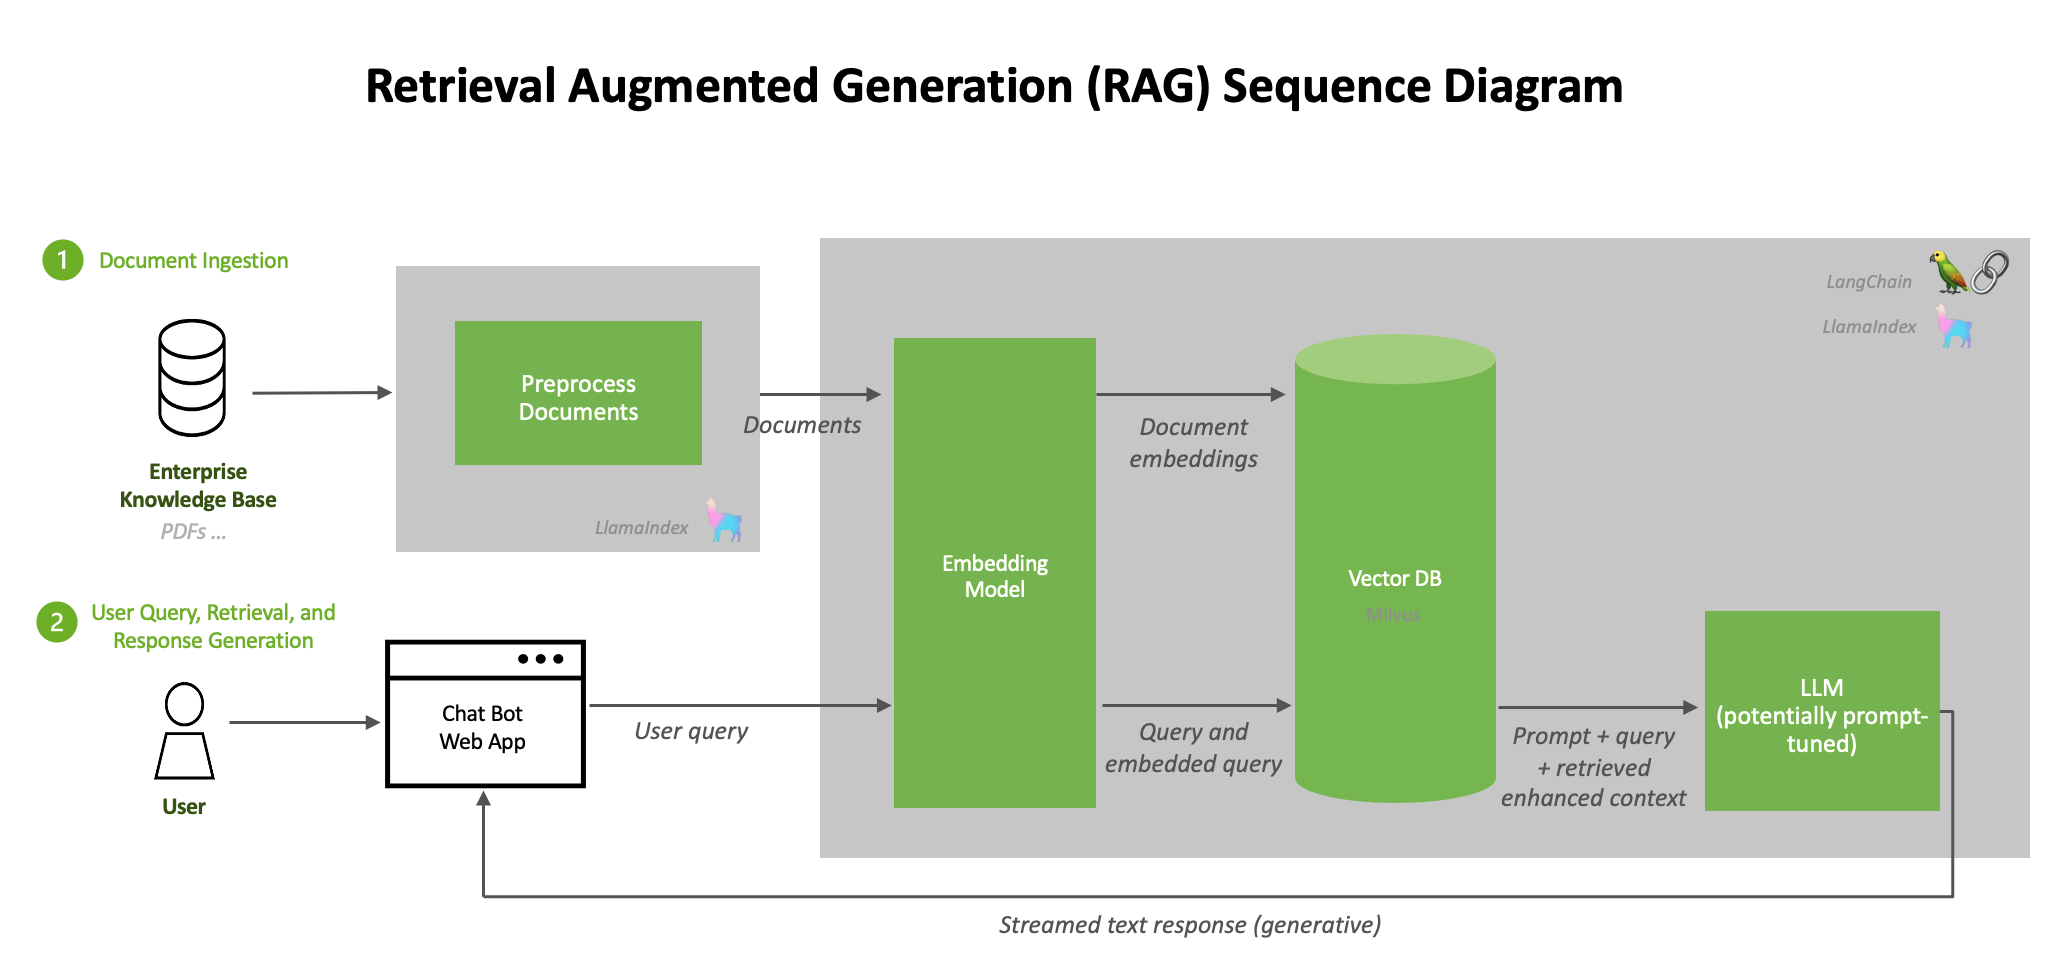
\includegraphics[width=1.0\textwidth]{rag_pipeline_diagram.png}
    \captionof{figure}{Sơ đồ kiến trúc của một hệ thống RAG, bao gồm giai đoạn Lập chỉ mục (bên trên) và giai đoạn Truy vấn (bên dưới).}
    \label{fig:rag_pipeline_diagram}
\end{center}

\subsection{Bài học từ các Công cụ Tìm kiếm: Kiến trúc Phân tầng của Google}
\label{ssec:lesson_from_google}
Để hiểu tại sao các hệ thống RAG hiện đại được thiết kế theo một cách cụ thể, sẽ rất hữu ích khi nhìn vào "người khổng lồ" trong lĩnh vực tìm kiếm: Google. Kiến trúc của Google Search là một ví dụ điển hình về một hệ thống retrieval đa tầng (multi-stage), nơi mỗi tầng sẽ lọc và tinh chỉnh kết quả, cân bằng giữa tốc độ và độ chính xác.

\paragraph{Kiến trúc Phân tầng (A Tiered Architecture)}
Một truy vấn trên Google không chỉ đơn giản là "tìm và trả về". Nó đi qua một "phễu" tinh vi gồm nhiều giai đoạn:
\begin{enumerate}
    \item \textbf{Crawl \& Indexing (Thu thập và Lập chỉ mục):} 
    Trước khi bất kỳ truy vấn nào được xử lý, Googlebot liên tục \emph{crawl} web, tải về nội dung và phân tích cấu trúc trang. Dữ liệu sau đó được chuẩn hoá và lưu trong nhiều loại chỉ mục:
    \begin{itemize}
        \item \emph{Inverted Index (Sparse Index):} ánh xạ từ khoá $\rightarrow$ danh sách tài liệu chứa từ đó.
        \item \emph{Dense Index (Vector Index):} biểu diễn văn bản dưới dạng embedding để phục vụ tìm kiếm ngữ nghĩa.
        \item Ngoài ra, các siêu dữ liệu (metadata), đồ thị liên kết (PageRank), và thông tin đa phương tiện (hình ảnh, video) cũng được lưu trữ song song.
    \end{itemize}

    \item \textbf{Query Understanding (Hiểu Truy vấn):} 
    Khi người dùng nhập một truy vấn, Google áp dụng các mô hình ngôn ngữ tiên tiến (BERT, MUM, T5) để phân tích ý định và ngữ nghĩa. Các bước xử lý điển hình gồm:
    \begin{itemize}
        \item Chuẩn hoá, sửa lỗi chính tả, mở rộng từ đồng nghĩa.
        \item Nhận diện thực thể (entity recognition) và giải quyết nhập nhằng (disambiguation).
        \item Viết lại truy vấn (query rewriting) và cá nhân hoá dựa trên ngôn ngữ, vị trí, lịch sử tìm kiếm.
    \end{itemize}

    \item \textbf{Candidate Generation (Tạo Ứng viên - Nhanh và Rộng):}
    \begin{itemize}
        \item \textbf{Mục tiêu:} Từ hàng tỷ tài liệu, nhanh chóng lọc ra một tập hợp lớn (10,000--100,000) ứng viên tiềm năng.
        \item \textbf{Công nghệ:} Kết hợp \emph{Sparse Retrieval} (BM25/TF-IDF) với \emph{Dense Retrieval} (bi-encoders + ANN search). Giai đoạn này ưu tiên \textbf{Recall} --- đảm bảo không bỏ sót kết quả quan trọng.
    \end{itemize}

    \item \textbf{Initial Ranking (Xếp hạng ban đầu):}
    \begin{itemize}
        \item \textbf{Mục tiêu:} Thu hẹp tập ứng viên từ hàng chục nghìn xuống còn vài nghìn tài liệu có triển vọng.
        \item \textbf{Công nghệ:} Sử dụng \emph{Learning-to-Rank models} (boosted trees, shallow neural nets) để kết hợp nhiều tín hiệu: điểm BM25, PageRank, độ mới (freshness), anchor text, độ phổ biến của tài liệu. Đây là lớp lọc trung gian quan trọng trước khi áp dụng mô hình ngôn ngữ nặng nề.
    \end{itemize}

    \item \textbf{Neural Re-ranking \& Final Touches (Xếp hạng lại bằng mô hình Neural và Tinh chỉnh cuối cùng):}
    \begin{itemize}
        \item \textbf{Mục tiêu:} Đạt độ chính xác cao nhất trong top kết quả hiển thị (thường là vài chục link).
        \item \textbf{Công nghệ:} Các \emph{Cross-Encoders} hoặc mô hình seq2seq (như T5, BERT, MUM) được áp dụng cho vài trăm ứng viên. Các mô hình này đánh giá trực tiếp cặp \emph{(truy vấn, tài liệu)} nên rất chính xác, dù tốn kém về tính toán.
        \item \textbf{Tinh chỉnh cuối cùng:} Diversification (đa dạng hoá kết quả), lọc spam, tích hợp Knowledge Graph, snippet, và kết hợp các nguồn media (tin tức, hình ảnh, video).
        \item Ngoài ra, các tín hiệu hành vi người dùng (CTR, dwell time) được khai thác để điều chỉnh thứ hạng theo thời gian.
    \end{itemize}
\end{enumerate}

\begin{tcolorbox}[
    title=Bài học cốt lõi cho RAG từ Google,
    colback=green!5!white, colframe=green!60!black, fonttitle=\bfseries
]
Xây dựng một hệ thống retrieval mạnh mẽ không phải là việc chọn một thuật toán duy nhất. Đó là việc xây dựng một \textbf{pipeline đa tầng}. Chúng ta chấp nhận sử dụng các phương pháp "đủ tốt" và nhanh ở giai đoạn đầu để lọc số lượng lớn, sau đó mới đầu tư tài nguyên tính toán vào các phương pháp chính xác cao cho một số lượng nhỏ các ứng viên hứa hẹn nhất. Triết lý "lọc rộng rồi tinh chỉnh sâu" này chính là nền tảng cho các hệ thống RAG hiện đại.
\end{tcolorbox}

\subsection{Tối ưu hóa Giai đoạn 1: Lập chỉ mục Thông minh (Smarter Indexing)}
\label{ssec:smarter_indexing}
Chất lượng của các chunk được lập chỉ mục ảnh hưởng trực tiếp đến khả năng tìm thấy thông tin chính xác. "Rác vào, Rác ra". Các kỹ thuật dưới đây giúp cải thiện "chất lượng đầu vào" cho hệ thống RAG.

\subsubsection{Chiến lược Phân mảnh Nâng cao (Advanced Chunking Strategies)}
Việc chia văn bản một cách "mù quáng" theo kích thước cố định (fixed-size chunking) thường làm phá vỡ ngữ nghĩa của câu hoặc đoạn văn.
\begin{itemize}
    \item \textbf{Chunking theo Ngữ nghĩa/Cấu trúc (Semantic/Structural Chunking):} Thay vì chia theo số ký tự, chúng ta chia dựa trên các ranh giới tự nhiên của văn bản như dấu ngắt câu, đoạn văn, tiêu đề (Markdown headers), hoặc các thẻ HTML. Điều này giúp các chunk giữ được sự mạch lạc và trọn vẹn về ý nghĩa.
    \item \textbf{Chunking có chồng lấn (Overlap Chunking):} Để tránh mất ngữ cảnh ở điểm nối giữa hai chunk, một phần nhỏ của chunk trước được lặp lại ở đầu chunk sau. Ví dụ: chunk 1 chứa các câu [1, 2, 3, 4], chunk 2 sẽ chứa các câu [4, 5, 6, 7].
\end{itemize}

\subsubsection{Kỹ thuật Small-to-Big và Sentence-Windowing}
Đây là một kỹ thuật mạnh mẽ để cân bằng giữa độ chính xác khi tìm kiếm và đầy đủ ngữ cảnh cho LLM.
\begin{itemize}
    \item \textbf{Vấn đề:} Các chunk lớn (nguyên đoạn văn) chứa nhiều ngữ cảnh nhưng khó khớp chính xác với một câu hỏi cụ thể. Các chunk nhỏ (một câu) thì dễ khớp chính xác nhưng lại thiếu ngữ cảnh xung quanh.
    \item \textbf{Giải pháp "Small-to-Big":}
    \begin{enumerate}
        \item \textbf{Lập chỉ mục (Index):} Chia tài liệu thành các đơn vị nhỏ (ví dụ: từng câu) và nhúng chúng.
        \item \textbf{Tìm kiếm (Retrieve):} Tìm kiếm trên các câu đơn lẻ để có độ chính xác cao nhất.
        \item \textbf{Mở rộng (Expand):} Sau khi tìm được câu phù hợp nhất, thay vì chỉ trả về câu đó, hệ thống sẽ lấy ra một "cửa sổ" văn bản lớn hơn xung quanh câu đó (ví dụ: 3 câu trước và 3 câu sau, hoặc toàn bộ đoạn văn chứa câu đó) để cung cấp cho LLM.
    \end{enumerate}
    Kỹ thuật này giúp đạt được \textit{sự chính xác trong tìm kiếm} và \textit{sự đầy đủ về ngữ cảnh} khi sinh câu trả lời.
\end{itemize}

\subsubsection{Tầm quan trọng của Metadata}
Metadata là "thông tin về thông tin". Khi lập chỉ mục, việc lưu trữ metadata cùng với mỗi chunk là cực kỳ quan trọng cho các ứng dụng thực tế.
\begin{itemize}
    \item \textbf{Ví dụ về Metadata:} Tên file nguồn, số trang, ngày xuất bản, tác giả, tiêu đề chương/mục, URL.
    \item \textbf{Tại sao nó quan trọng?}
    \begin{itemize}
        \item \textbf{Trích dẫn nguồn:} Giúp LLM có thể trích dẫn nguồn gốc của thông tin một cách chính xác trong câu trả lời (ví dụ: "Theo tài liệu X, trang 5...").
        \item \textbf{Lọc trước khi tìm kiếm (Pre-filtering):} Cho phép thu hẹp không gian tìm kiếm. Ví dụ: "Chỉ tìm kiếm trong các tài liệu được xuất bản sau năm 2023".
        \item \textbf{Gỡ lỗi (Debugging):} Dễ dàng truy vết xem chunk gây ra câu trả lời sai đến từ tài liệu nào.
    \end{itemize}
\end{itemize}

\subsection{Tối ưu hóa Giai đoạn 2: Tìm kiếm và Xếp hạng (Advanced Retrieval \& Ranking)}
\label{ssec:advanced_retrieval_ranking}
\begin{tcolorbox}[title=Mục tiêu, colback=blue!5!white, colframe=blue!75!black]
Retriever là trái tim của RAG. Giai đoạn này quyết định "chất lượng nguyên liệu đầu vào" cho LLM. Một hệ thống RAG chỉ có thể tốt bằng thành phần retriever của nó. Các kỹ thuật dưới đây giúp tìm được những mảnh ghép thông tin (chunk) chính xác, liên quan và đa dạng nhất.
\end{tcolorbox}

\subsection{Tối ưu hóa Giai đoạn 2: Tìm kiếm và Xếp hạng (Advanced Retrieval \& Ranking)}
\label{ssec:advanced_retrieval_ranking_refactored}
Lấy cảm hứng từ kiến trúc của Google, giờ đây chúng ta sẽ áp dụng triết lý đa tầng vào hệ thống RAG của mình.

\subsubsection{Tìm kiếm Lai (Hybrid Search): Giai đoạn Candidate Generation của RAG}
Đây chính là giai đoạn 1 của chúng ta. Thay vì chỉ dùng một phương pháp, ta kết hợp cả hai:
\begin{itemize}
    \item \textbf{Cơ chế:} Hệ thống chạy song song cả Sparse Retriever (BM25) và Dense Retriever (Vector Search). Sau đó, điểm số từ hai hệ thống được kết hợp lại (ví dụ: dùng thuật toán Reciprocal Rank Fusion - RRF) để tạo ra một danh sách ứng viên (candidate list) chất lượng cao.
    \item \textbf{Lợi ích:} Tận dụng khả năng khớp từ khóa chính xác của Sparse và khả năng hiểu ngữ nghĩa sâu sắc của Dense. Đây được coi là phương pháp mặc định để có được recall tốt nhất.
\end{itemize}

\subsubsection{Xếp hạng lại (Re-ranking) với Cross-Encoders}
\begin{itemize}
    \item \textbf{Vấn đề:} Hybrid Search rất nhanh và hiệu quả để lọc ra top 100-200 ứng cử viên tiềm năng từ hàng triệu chunk. Nhưng trong top 100 này, đâu mới là những chunk thực sự tốt nhất?
    \item \textbf{Giải pháp:} Sử dụng một mô hình thứ hai, mạnh hơn nhưng chậm hơn, gọi là \textbf{Cross-Encoder}.
        \begin{itemize}
            \item \textbf{Cơ chế:} Thay vì tạo vector riêng cho câu hỏi và tài liệu, Cross-Encoder nhận vào cặp \texttt{(câu hỏi, chunk)} và đưa ra một điểm số tương đồng duy nhất. Việc xem xét cả hai cùng lúc cho phép nó hiểu được sự tương tác tinh vi hơn.
            \item \textbf{Quy trình:} Hybrid Search tìm ra top-K ứng viên (K lớn). Sau đó, Cross-Encoder sẽ đánh giá và xếp hạng lại top-K này để chọn ra top-N cuối cùng (N nhỏ) gửi cho LLM.
        \end{itemize}
\end{itemize}

\subsection{Tối ưu hóa Giai đoạn 3: Tăng cường và Sinh (Smarter Augmentation \& Generation)}
\label{ssec:smarter_aug_gen}
Sau khi đã có những chunk chất lượng nhất, chúng ta cần đảm bảo chúng được sử dụng một cách hiệu quả và trung thực.

\subsubsection{Nén Ngữ cảnh (Context Compression)}
Đôi khi, các chunk được tìm thấy vẫn chứa nhiều thông tin thừa so với câu hỏi. Việc "nhồi nhét" tất cả vào prompt có thể làm LLM bị nhiễu.
\begin{itemize}
    \item \textbf{Cơ chế:} Trước khi đưa các chunk vào prompt cuối cùng, một mô hình nhỏ hơn sẽ chạy qua và chỉ giữ lại những câu, những ý có liên quan trực tiếp đến câu hỏi của người dùng.
    \item \textbf{Lợi ích:} Giảm độ dài của prompt (tiết kiệm chi phí), tăng sự tập trung cho LLM vào các bằng chứng quan trọng nhất.
\end{itemize}

\subsubsection{Kiểm soát việc Sinh: Buộc Trích dẫn và Chống Bịa đặt (Hallucination Guardrails)}
Đây là bước cuối cùng và quan trọng nhất để đảm bảo tính tin cậy.
\begin{itemize}
    \item \textbf{Instruction Tuning:} Huấn luyện hoặc chỉ dẫn LLM một cách rõ ràng thông qua prompt: \textit{"Hãy trả lời câu hỏi chỉ dựa trên ngữ cảnh được cung cấp. Với mỗi thông tin đưa ra, hãy trích dẫn nguồn [doc\_id, chunk\_id]. Nếu thông tin không có trong ngữ cảnh, hãy trả lời 'Tôi không tìm thấy thông tin trong tài liệu'."}
    \item \textbf{Giảm Temperature:} Khi sinh câu trả lời, đặt tham số `temperature` của LLM ở mức thấp (ví dụ: 0.1) để giảm tính ngẫu nhiên và sáng tạo, buộc nó bám sát vào văn bản nguồn.
\end{itemize}

\subsection{Các Mô hình RAG Nâng cao (Advanced RAG Patterns)}
\label{ssec:advanced_rag_patterns}
Khi các bài toán trở nên phức tạp hơn, chúng ta cần các kiến trúc RAG tinh vi hơn.

\begin{itemize}
    \item \textbf{Biến đổi Truy vấn (Query Transformation):} Câu hỏi của người dùng thường không phải là dạng tốt nhất để tìm kiếm. Các kỹ thuật này sẽ biến đổi nó trước:
        \begin{itemize}
        \item \textbf{Viết lại Truy vấn (Query Rewriting):} Là nhóm kỹ thuật tập trung vào việc sửa đổi, mở rộng, hoặc diễn đạt lại văn bản câu hỏi gốc mà không làm thay đổi ý định tìm kiếm cốt lõi. Mục tiêu là cải thiện sự tương thích giữa từ vựng của người dùng và từ vựng trong kho tài liệu, qua đó tăng cả \textit{recall} và \textit{precision}. Các phương pháp này được chia thành ba hướng tiếp cận chính:
    
        \begin{itemize}
            \item \textbf{Viết lại dựa trên Từ vựng (Lexical Rewriting):} 
            Các phương pháp này hoạt động ở cấp độ từ hoặc ký tự, dựa trên các quy tắc, từ điển, hoặc các chuẩn hóa ngôn ngữ cơ bản.
            \begin{itemize}
                \item \textbf{Mở rộng Từ đồng nghĩa (Synonym/Thesaurus Expansion):} Bổ sung các từ hoặc cụm từ đồng nghĩa (ví dụ: \texttt{luật pháp} $\rightarrow$ \texttt{pháp luật}, \texttt{quy định}) để tăng khả năng khớp, giúp bắt được các tài liệu sử dụng cách diễn đạt khác nhau.
                \item \textbf{Chuẩn hóa Hình thái học (Morphological Normalization):} Đưa các biến thể của một từ về dạng gốc (stemming hoặc lemmatization). Ví dụ: các từ \texttt{xử lý}, \texttt{được xử lý}, \texttt{sự xử lý} đều được đưa về gốc \texttt{xử lý}.
                \item \textbf{Sửa lỗi Chính tả/Gõ nhầm (Spelling/Typo Correction):} Tự động phát hiện và sửa các lỗi sai trong truy vấn (\texttt{luật lao đông} $\rightarrow$ \texttt{luật lao động}) để tránh tìm kiếm thất bại.
                \item \textbf{Mở rộng Từ viết tắt (Abbreviation Expansion):} Chuyển các từ viết tắt thành dạng đầy đủ của chúng (ví dụ: \texttt{TP.HCM} $\rightarrow$ \texttt{Thành phố Hồ Chí Minh}, \texttt{LHQ} $\rightarrow$ \texttt{Liên Hợp Quốc}).
                \item \textbf{Xử lý Stopword (Stopword Handling):} Loại bỏ các từ phổ biến, ít mang nghĩa (như \texttt{là}, \texttt{của}, \texttt{và}) để tập trung vào từ khóa chính, hoặc ngược lại, giữ lại chúng khi cần thiết cho các truy vấn yêu cầu sự chính xác về ngữ pháp (phrase queries).
            \end{itemize}
    
            \item \textbf{Viết lại dựa trên Thống kê (Statistical Rewriting):} 
            Các kỹ thuật này tận dụng thông tin thống kê từ kho tài liệu hoặc từ kết quả tìm kiếm ban đầu để mở rộng truy vấn một cách tự động.
            \begin{itemize}
                \item \textbf{Phản hồi Giả liên quan (Pseudo-Relevance Feedback - PRF):} Giả định rằng các tài liệu top-k trong kết quả tìm kiếm ban đầu là liên quan. Hệ thống sẽ trích xuất các thuật ngữ quan trọng từ các tài liệu này để bổ sung vào truy vấn gốc và thực hiện tìm kiếm lại. (Các thuật toán tiêu biểu: Rocchio, RM3).
                \item \textbf{Mở rộng dựa trên Tần suất Cùng xuất hiện (Term Co-occurrence Expansion):} Tìm và thêm vào truy vấn các thuật ngữ thường xuyên xuất hiện cùng với các thuật ngữ gốc trong toàn bộ kho tài liệu (Dựa trên các độ đo như Pointwise Mutual Information - PMI).
                \item \textbf{Mở rộng dựa trên Mô hình Chủ đề (Topic-Model-Based Expansion):} Sử dụng các mô hình như LDA (Latent Dirichlet Allocation) để xác định các chủ đề chính của truy vấn, sau đó bổ sung các từ khóa đặc trưng của những chủ đề đó.
                \item \textbf{Mô hình Liên quan (Relevance Models):} Ước tính một mô hình xác suất của các thuật ngữ sẽ xuất hiện trong một tài liệu liên quan, sau đó lấy mẫu từ mô hình này để tạo ra truy vấn mới.
            \end{itemize}
            
            \item \textbf{Viết lại dựa trên Ngữ nghĩa (Semantic Rewriting):} 
            Các phương pháp hiện đại, tập trung vào việc nắm bắt và mở rộng ý nghĩa, ngữ cảnh của truy vấn thay vì chỉ dựa trên từ vựng bề mặt.
            \begin{itemize}
                \item \textbf{Dựa trên Vector Embedding (Embedding-based Nearest Neighbors):} Biểu diễn truy vấn dưới dạng vector và tìm các từ/cụm từ có vector gần nhất trong không gian embedding để mở rộng (Ví dụ: sử dụng Word2Vec, GloVe, fastText).
                \item \textbf{Diễn đạt lại bằng LLM (LLM-based Paraphrasing):} Sử dụng các mô hình ngôn ngữ lớn (LLM) như GPT-4 hay T5 để tạo ra một phiên bản câu hỏi hoàn toàn mới nhưng giữ nguyên ý nghĩa, giúp vượt qua rào cản từ vựng.
                \item \textbf{Tạo nhiều Truy vấn song song (Multi-Query Rewriting):} Yêu cầu LLM sinh ra nhiều biến thể khác nhau của câu hỏi gốc. Hệ thống sẽ thực hiện tìm kiếm với tất cả các biến thể này và tổng hợp kết quả.
                \item \textbf{Mở rộng bằng Đồ thị Tri thức (Knowledge-Graph Expansion):} Liên kết các thực thể trong truy vấn (tên người, địa điểm, tổ chức) với một đồ thị tri thức. Sau đó, mở rộng truy vấn bằng cách thêm vào các thông tin, thuộc tính, hoặc các thực thể liên quan được lấy từ đồ thị.
                \item \textbf{Mở rộng theo Ngữ cảnh Hội thoại (Contextual Expansion):} Tận dụng lịch sử của cuộc trò chuyện để làm rõ và bổ sung thông tin cho truy vấn hiện tại. Ví dụ, câu hỏi "còn anh ấy thì sao?" sẽ được mở rộng với thông tin về "anh ấy" đã được đề cập trước đó.
            \end{itemize}
        \end{itemize}
        \item \textbf{Biến đổi Biểu diễn Truy vấn (Query Representation Transformation):} Khác với việc viết lại văn bản, nhóm kỹ thuật này giữ nguyên câu hỏi gốc nhưng biến đổi cách nó được \textit{biểu diễn} (thường là dưới dạng vector) để tối ưu hóa việc so khớp trong không gian embedding.
        \begin{itemize}
            \item \textbf{HyDE (Hypothetical Document Embeddings):} 
            Một kỹ thuật đột phá, yêu cầu LLM tự sinh một tài liệu trả lời \textit{giả định} cho câu hỏi. Thay vì nhúng vector của câu hỏi ngắn gọn và thiếu ngữ cảnh, hệ thống sẽ nhúng vector của tài liệu giả định này. Vector này thường giàu thông tin và nằm gần các tài liệu liên quan thực tế trong không gian embedding, do đó cải thiện đáng kể chất lượng tìm kiếm.
            
            \item \textbf{Query2Doc (Q2D):} 
            Một phương pháp tiền thân của HyDE, cũng biến đổi truy vấn thành một dạng trông giống tài liệu hơn, nhưng thường sử dụng các phương pháp heuristic hoặc các mô hình sinh văn bản gọn nhẹ (như T5) thay vì các LLM lớn.
            
            \item \textbf{Tăng cường Embedding Truy vấn (Query Embedding Augmentation):} 
            Cải thiện vector truy vấn gốc bằng cách kết hợp nó với các thông tin bổ sung.
            \begin{itemize}
                \item \textbf{Pooling với các Mở rộng (Average Pooling with Expansions):} 
                Tạo embedding cho truy vấn gốc và các phiên bản mở rộng (ví dụ: từ đồng nghĩa), sau đó kết hợp chúng lại (ví dụ: lấy trung bình) để tạo ra một vector đại diện toàn diện hơn.
                \item \textbf{Hợp nhất Embedding (Embedding Fusion):} 
                Thực hiện tìm kiếm song song với nhiều hệ thống retriever (ví dụ: một sparse retriever như BM25 và một dense retriever). Sau đó, vector truy vấn cuối cùng được điều chỉnh hoặc kết hợp dựa trên thông tin từ các kết quả tìm kiếm này.
            \end{itemize}
            
            \item \textbf{Biểu diễn Truy vấn Tương phản (Contrastive Query Representation):} 
            Tinh chỉnh (fine-tune) mô hình encoder để nó học được cách tạo ra các embedding tốt hơn. Cụ thể, mô hình được huấn luyện để vector của truy vấn gần với vector của tài liệu trả lời đúng (positive sample) và xa các tài liệu không liên quan (negative samples).
            
            \item \textbf{Biến đổi Ngầm định qua Kiến trúc (Implicit Transformation via Architecture):} 
            Một số kiến trúc retriever không tạo ra một vector duy nhất cho truy vấn. Thay vào đó, chúng thực hiện một sự biến đổi ngầm thông qua tương tác sâu hơn giữa truy vấn và tài liệu.
            \begin{itemize}
                \item \textbf{ColBERT (Late Interaction):} 
                Mô hình này tạo ra embedding cho mỗi token trong cả truy vấn và tài liệu. Quá trình so khớp tính toán điểm tương đồng giữa mỗi token của truy vấn với tất cả các token của tài liệu, cho phép một sự tương tác chi tiết và linh hoạt hơn là so khớp hai vector đơn lẻ.
            \end{itemize}
        \end{itemize}
    
        \item \textbf{Phân tích và Cấu trúc hóa Truy vấn (Query Understanding \& Structuring):} Nhóm kỹ thuật này không chỉ "hiểu" ý định của truy vấn mà còn "dịch" nó thành một định dạng có cấu trúc, cho phép tìm kiếm chính xác trên các nguồn dữ liệu có schema rõ ràng (structured/semi-structured data) như cơ sở dữ liệu hoặc kho tri thức.
        \begin{itemize}
            \item \textbf{Tự truy vấn (Self-Querying):} 
            LLM được cung cấp thông tin về siêu dữ liệu (metadata) của kho tài liệu (ví dụ: \texttt{năm xuất bản}, \texttt{tác giả}, \texttt{thể loại}). Khi nhận câu hỏi, LLM tự động phân tích và trích xuất các bộ lọc tương ứng. Ví dụ, câu hỏi "các bài báo của Hinton về mạng nơ-ron sau 2015" sẽ được dịch thành một truy vấn tìm kiếm nội dung "mạng nơ-ron" kèm theo hai bộ lọc: \texttt{tác giả = "Hinton"} và \texttt{năm > 2015}.
            
            \item \textbf{Phân tích Ngữ nghĩa (Semantic Parsing):} 
            Chuyển đổi hoàn toàn câu hỏi ngôn ngữ tự nhiên thành một truy vấn trong một ngôn ngữ truy vấn chính thức như SQL (cho cơ sở dữ liệu quan hệ), SPARQL (cho đồ thị tri thức), hoặc GraphQL.
            
            \item \textbf{Phân rã Truy vấn (Query Decomposition / Multi-Hop):} 
            Đối với các câu hỏi phức tạp đòi hỏi phải kết hợp thông tin từ nhiều nguồn, kỹ thuật này chia câu hỏi lớn thành một chuỗi các câu hỏi con đơn giản hơn. Kết quả của câu hỏi con trước được dùng làm đầu vào cho câu hỏi con tiếp theo.
            
            \item \textbf{Phân định Nghĩa (Query Disambiguation):} 
            Xác định ý nghĩa chính xác của các từ đa nghĩa dựa trên ngữ cảnh. Ví dụ, hệ thống cần phân biệt "Apple" là công ty công nghệ hay là một loại trái cây để có thể tìm kiếm đúng hướng.
            
            \item \textbf{Phân loại Ý định và Trích xuất Thực thể (Intent Classification \& Slot Filling):} 
            Một cách tiếp cận phổ biến trong các hệ thống chatbot, trong đó hệ thống xác định mục đích chung của người dùng (intent) và trích xuất các thông tin chi tiết (entities/slots). Ví dụ, trong câu "đặt vé máy bay đến Hà Nội vào ngày mai", intent là "đặt vé", và các slot là \texttt{đích đến = "Hà Nội"} và \texttt{thời gian = "ngày mai"}.
            
            \item \textbf{Phân loại theo Khía cạnh (Query Faceting):} 
            Tự động nhận diện và tách câu hỏi thành nhiều khía cạnh hoặc thuộc tính khác nhau, thường được dùng trong các hệ thống tìm kiếm thương mại điện tử. Ví dụ, truy vấn "điện thoại Samsung dưới 10 triệu pin trâu" có thể được tách thành các facet: \texttt{thương hiệu = "Samsung"}, \texttt{giá < 10,000,000 VNĐ}, \texttt{tính năng = "pin dung lượng cao"}.
        \end{itemize}
        
        \item \textbf{Viết lại Truy vấn dựa trên Học máy (Learning-based Query Rewriting):} Nhóm kỹ thuật này coi việc tạo ra truy vấn tối ưu là một bài toán cần học từ dữ liệu, thay vì dựa trên các quy tắc hoặc heuristic cố định. Các mô hình được huấn luyện để tự động tạo ra các phiên bản truy vấn hiệu quả nhất.
        \begin{itemize}
            \item \textbf{Viết lại dựa trên Học tăng cường (Reinforcement Learning - RL):} 
            Xây dựng một "tác nhân" (agent) thông minh có khả năng ra quyết định viết lại truy vấn thông qua thử và sai. Agent học một "chính sách" (policy) để tạo ra các truy vấn tốt nhất dựa trên "phần thưởng" (reward) nhận được từ môi trường.
            \begin{itemize}
                \item \textbf{Học để Truy xuất (Learning to Retrieve with RL):} 
                Phần thưởng được tính trực tiếp dựa trên chất lượng của tập tài liệu truy xuất được (ví dụ: recall, precision, MRR). Agent được khuyến khích tạo ra các truy vấn tìm thấy nhiều tài liệu liên quan hơn.
                
                \item \textbf{RL dựa trên Chất lượng Câu trả lời (Answer-based RL):} 
                Một cách tiếp cận sâu hơn, trong đó phần thưởng không chỉ dựa trên kết quả truy xuất mà còn dựa trên chất lượng của câu trả lời cuối cùng do mô hình sinh tạo ra. Điều này giúp tối ưu toàn bộ pipeline RAG một cách end-to-end.
                
                \item \textbf{Viết lại Chủ động (Active Query Rewriting):} 
                Agent có khả năng tự quyết định xem có cần thực hiện thêm một bước viết lại nữa hay không. Nếu kết quả tìm kiếm ban đầu đã tốt, agent có thể dừng lại để tiết kiệm tài nguyên tính toán.
                
                \item \textbf{Học theo Lộ trình (Curriculum RL):} 
                Agent được huấn luyện theo một lộ trình có cấu trúc, bắt đầu từ những câu hỏi đơn giản và dần dần tăng độ khó. Cách tiếp cận này giúp agent học các chiến lược viết lại một cách ổn định và hiệu quả hơn.
                
                \item \textbf{Học Tương tác (Interactive RL):} 
                Tận dụng phản hồi trực tiếp từ người dùng (ví dụ: nhấn "thích" hoặc báo cáo kết quả không chính xác) như một nguồn tín hiệu phần thưởng bổ sung, giúp agent cá nhân hóa và thích ứng nhanh chóng.
                
                \item \textbf{Học Phân cấp (Hierarchical RL):} 
                Sử dụng một kiến trúc RL đa tầng. Một "meta-agent" cấp cao sẽ quyết định \textit{loại} chiến lược viết lại cần dùng (ví dụ: mở rộng từ đồng nghĩa, thêm bộ lọc, hay phân rã câu hỏi), trong khi một agent cấp thấp sẽ thực thi chi tiết chiến lược đó.
            \end{itemize}
            
            \item \textbf{Truy xuất Khả vi End-to-End (End-to-End Differentiable Retrieval):} 
            Các phương pháp này tích hợp bộ phận retriever vào trong quá trình huấn luyện của mô hình ngôn ngữ lớn, cho phép tối ưu hóa việc biểu diễn truy vấn một cách trực tiếp.
            \begin{itemize}
                \item \textbf{Học Biểu diễn Truy vấn (DPR, ColBERT, Retro):} 
                Encoder của truy vấn được huấn luyện trực tiếp từ tín hiệu lỗi (loss) của tác vụ cuối cùng (ví dụ: trả lời câu hỏi). Quá trình này "ép" mô hình phải học cách tạo ra các embedding truy vấn hiệu quả nhất cho tác vụ đó.
                \item \textbf{Huấn luyện Tăng cường Truy xuất (Retrieval-Augmented Training):} 
                Các mô hình như RAG hay Atlas tối ưu đồng thời cả retriever và generator. Retriever học cách tìm kiếm tài liệu hữu ích, và generator học cách tận dụng các tài liệu đó để sinh ra câu trả lời tốt hơn, tạo thành một vòng lặp tối ưu hóa lẫn nhau.
            \end{itemize}
        \end{itemize}
    
        \item \textbf{Định tuyến và Biến đổi Meta (Query Routing \& Meta-Transformation):}
            Trong các hệ thống RAG phức tạp sử dụng nhiều công cụ hoặc nhiều nguồn dữ liệu, nhóm kỹ thuật này đóng vai trò như một "bộ điều phối" thông minh, quyết định cách xử lý truy vấn một cách hiệu quả nhất.
            \begin{itemize}
                \item \textbf{Định tuyến Truy vấn (Query Routing):} 
                Dựa trên nội dung của câu hỏi, hệ thống sẽ quyết định gửi nó đến retriever phù hợp nhất. Ví dụ, các câu hỏi chứa từ khóa rõ ràng có thể được gửi đến BM25 (sparse), trong khi các câu hỏi trừu tượng hơn sẽ được gửi đến dense retriever. Tương tự, hệ thống có thể định tuyến truy vấn đến các kho tri thức chuyên ngành khác nhau (ví dụ: y tế, pháp luật).
                
                \item \textbf{Tái định dạng Truy vấn cho Công cụ (Query Reformulation for Tools):} 
                Trong các hệ thống RAG dựa trên agent, LLM đóng vai trò trung tâm, có khả năng tự biến đổi câu hỏi của người dùng thành các lời gọi hàm hoặc các truy vấn API hợp lệ để tương tác với các công cụ bên ngoài (ví dụ: công cụ tìm kiếm web, máy tính, API thời tiết).
                
                \item \textbf{Hợp nhất Truy vấn (Query Fusion):} 
                Thay vì chọn một retriever duy nhất, hệ thống gửi truy vấn đến nhiều retriever song song và sau đó thông minh hợp nhất các kết quả lại. Các phương pháp phổ biến bao gồm bỏ phiếu (voting), hợp nhất có trọng số (weighted fusion), hoặc Reciprocal Rank Fusion (RRF).
                
                \item \textbf{Chiến lược Truy vấn Thích ứng (Adaptive Query Strategy):} 
                Đây là một phương pháp động, trong đó hệ thống tự quyết định chiến lược biến đổi nào là tốt nhất cho một truy vấn cụ thể tại một thời điểm nhất định. Ví dụ, hệ thống có thể thử một truy vấn mở rộng đơn giản trước, nếu kết quả không tốt, nó sẽ tự động chuyển sang một chiến lược phức tạp hơn như HyDE hoặc phân rã câu hỏi (multi-hop).
            \end{itemize}
        
        \end{itemize}
    \item \textbf{RAG Đa bước (Multi-Hop RAG):}
    Được thiết kế để giải quyết các câu hỏi phức tạp đòi hỏi phải suy luận theo chuỗi (reasoning chain) và tổng hợp bằng chứng từ nhiều tài liệu hoặc nguồn thông tin khác nhau. Thay vì một lần truy xuất duy nhất, hệ thống thực hiện nhiều "bước nhảy" (hops) để thu thập đủ thông tin cần thiết.
    
    Ví dụ, với câu hỏi: \textit{"Thủ tướng Anh hiện tại có quan điểm gì về chính sách của tổng thống Pháp?"}, một hệ thống multi-hop sẽ không tìm kiếm trực tiếp mà sẽ phân rã và thực hiện theo các bước. Các phương pháp để thực hiện điều này rất đa dạng:

    \begin{itemize}
        \item \textbf{Dựa trên Phân rã (Decomposition-based):} 
        Đây là hướng tiếp cận trực tiếp nhất, trong đó câu hỏi phức tạp được chia thành các câu hỏi con đơn giản hơn.
        \begin{itemize}
            \item \textbf{Phân rã Truy vấn (Query Decomposition):} 
            Sử dụng LLM để tự động phân rã câu hỏi gốc. Ví dụ trên sẽ được chia thành: (1) "Thủ tướng Anh hiện tại là ai?", (2) "Tổng thống Pháp hiện tại là ai?", và (3) "Quan điểm của [kết quả 1] về chính sách của [kết quả 2] là gì?".
            \item \textbf{Truy xuất Lặp (Iterative Retrieval):} 
            Hệ thống thực hiện truy xuất tuần tự. Kết quả của bước truy xuất trước được sử dụng để tạo ra câu hỏi cho bước tiếp theo. Đây chính là cơ chế hoạt động cốt lõi của ví dụ về thủ tướng Anh - tổng thống Pháp.
        \end{itemize}

        \item \textbf{Dựa trên Đồ thị (Graph-based):} 
        Phương pháp này biến đổi toàn bộ kho tài liệu thành một Đồ thị Tri thức (Knowledge Graph), trong đó các thực thể là các nút (nodes) và mối quan hệ là các cạnh (edges).
        \begin{itemize}
            \item \textbf{Tìm kiếm Đường đi (Path Finding):} 
            Câu hỏi của người dùng được chuyển thành một bài toán tìm đường đi trên đồ thị. Ví dụ: "Ai đã đạo diễn bộ phim mà Tom Hanks đóng vai chính?" sẽ trở thành việc tìm một đường đi từ nút \texttt{Tom Hanks} đến một nút \texttt{Đạo diễn} thông qua một nút \texttt{Bộ phim}. (Phương pháp này rất phổ biến trong các bộ dữ liệu QA phức tạp như HotpotQA).
        \end{itemize}

        \item \textbf{Tăng cường bằng Suy luận (Reasoning-augmented):} 
        Các phương pháp này tích hợp chặt chẽ quá trình suy luận của LLM vào vòng lặp truy xuất, làm cho quá trình tìm kiếm trở nên linh hoạt và thông minh hơn.
        \begin{itemize}
            \item \textbf{Chain-of-Thought (CoT) RAG:} 
            LLM thực hiện suy luận từng bước một ("think out loud"). Tại mỗi bước, nếu thấy thiếu thông tin, nó sẽ chủ động tạo ra một truy vấn con để gửi đến retriever, sau đó sử dụng kết quả để tiếp tục chuỗi suy luận.
            \item \textbf{Tree-of-Thoughts / Graph-of-Thoughts RAG:} 
            Thay vì một chuỗi suy luận tuyến tính duy nhất, hệ thống tạo ra và khám phá nhiều nhánh suy luận song song. Nếu một nhánh đi vào ngõ cụt, hệ thống có thể quay lại và thử một hướng khác, giúp tăng cường sự mạnh mẽ và khả năng tìm ra lời giải cho các câu hỏi cực kỳ phức tạp.
        \end{itemize}

        \item \textbf{Tăng cường bằng Bộ nhớ (Memory-augmented):} 
        Được thiết kế để giải quyết các chuỗi suy luận dài, nơi việc duy trì ngữ cảnh là tối quan trọng.
        \begin{itemize}
            \item \textbf{Bộ nhớ Làm việc (Working Memory):} 
            Mỗi kết quả trung gian, bằng chứng, hoặc suy luận được sinh ra trong quá trình multi-hop sẽ được lưu vào một "bộ nhớ đệm" hoặc "bảng nháp" (scratchpad). Tại các bước sau, LLM có thể tham chiếu lại thông tin trong bộ nhớ này, giúp tránh truy xuất lại thông tin đã có, giữ ngữ cảnh xuyên suốt, và cho phép thực hiện các chuỗi suy luận dài và phức tạp hơn.
        \end{itemize}
    \end{itemize}
    \item \textbf{RAG dạng Tác tử (Agentic RAG):}
    Đây là một bước tiến hóa của RAG, nơi LLM không còn là một thành phần thụ động trong một pipeline cố định mà trở thành một "tác tử" (agent) tự chủ, có khả năng lập kế hoạch, ra quyết định và thực thi một chiến lược truy xuất linh hoạt. Thay vì chỉ trả lời dựa trên những gì được cung cấp, agent sẽ chủ động điều khiển toàn bộ quá trình thu thập thông tin.

    \begin{itemize}
        \item \textbf{RAG Tăng cường bằng Công cụ (Tool-augmented RAG):} 
        LLM được trao quyền truy cập vào một bộ công cụ đa dạng, không chỉ giới hạn ở một retriever duy nhất. Dựa vào bản chất của câu hỏi, agent có thể tự quyết định:
        \begin{itemize}
            \item Khi nào cần gọi đến retriever nội bộ (để tìm trong kho tri thức).
            \item Khi nào cần sử dụng công cụ tìm kiếm bên ngoài (như Google Search) để lấy thông tin mới nhất.
            \item Khi nào cần truy vấn một cơ sở dữ liệu có cấu trúc (qua SQL).
            \item Khi nào cần sử dụng một công cụ tính toán (calculator) cho các câu hỏi số học.
        \end{itemize}

        \item \textbf{Truy xuất Thích ứng (Adaptive Retrieval):} 
        Agent có khả năng điều chỉnh chiến lược truy xuất một cách linh hoạt ngay trong quá trình xử lý một câu hỏi, thay vì tuân theo một quy trình cứng nhắc.
        \begin{itemize}
            \item \textbf{Độ sâu Truy xuất Động (Dynamic Retrieval Depth):} 
            Sau khi truy xuất một vài tài liệu ban đầu, agent tự đánh giá xem thông tin đã đủ để trả lời hay chưa. Nếu chưa, nó sẽ quyết định truy xuất thêm; nếu đủ, nó sẽ dừng lại để tiết kiệm tài nguyên.
            \item \textbf{Lựa chọn/Định tuyến Retriever (Retriever Selection/Routing):} 
            Agent phân tích câu hỏi và chọn công cụ retriever phù hợp nhất từ nhiều lựa chọn có sẵn: dùng BM25 cho các truy vấn dựa trên từ khóa, dùng dense retriever cho các câu hỏi ngữ nghĩa, hoặc dùng retriever trên đồ thị tri thức cho các câu hỏi về mối quan hệ.
        \end{itemize}

        \item \textbf{Kiến trúc Lập kế hoạch - Thực thi (Planner-Executor Framework):} 
        Tách biệt quá trình tư duy và hành động.
        \begin{itemize}
            \item \textbf{Planner (Người lập kế hoạch):} 
            LLM phân tích câu hỏi phức tạp và tạo ra một kế hoạch hành động từng bước. Ví dụ: "Đầu tiên, tìm thông tin về A. Sau đó, dùng kết quả đó để tìm thông tin về B. Cuối cùng, tổng hợp cả hai để trả lời."
            \item \textbf{Executor (Người thực thi):} 
            Một thành phần khác (hoặc chính LLM trong một vai trò khác) sẽ thực hiện từng bước trong kế hoạch (gọi tool, truy vấn retriever) và trả kết quả về cho Planner. Planner sẽ cập nhật kế hoạch dựa trên kết quả mới nhận được.
        \end{itemize}

        \item \textbf{RAG Tác tử Tương tác (Interactive Agentic RAG):} 
        Agent có khả năng tương tác với người dùng để cải thiện quá trình tìm kiếm, tạo ra một vòng lặp phản hồi (human-in-the-loop).
        \begin{itemize}
            \item \textbf{Làm rõ Truy vấn (Query Clarification):} 
            Nếu câu hỏi của người dùng mơ hồ hoặc không đủ chi tiết, thay vì đoán mò, agent sẽ chủ động đặt câu hỏi ngược lại để làm rõ. Ví dụ: "Khi bạn nói về 'Apple', bạn đang muốn hỏi về công ty công nghệ hay về một loại trái cây?"
        \end{itemize}

        \item \textbf{RAG Tác tử Tăng cường bằng Học máy (Learning-enhanced Agentic RAG):} 
        Chiến lược ra quyết định của agent không phải là cố định mà có thể được cải thiện thông qua học máy, đặc biệt là Học tăng cường (RL).
        \begin{itemize}
            \item \textbf{Học Chính sách Truy xuất (Learning Retrieval Policies):} 
            Agent học được một "chính sách" (policy) tối ưu qua thời gian. Ví dụ, nó có thể học được rằng: "Với các câu hỏi so sánh, chiến lược multi-hop thường hiệu quả hơn", hoặc "Khi người dùng hỏi về tin tức, hãy ưu tiên sử dụng công cụ tìm kiếm web".
        \end{itemize}
    \end{itemize}
\end{itemize}

\subsection{Đánh giá và Triển khai Hệ thống RAG}
\label{ssec:rag_evaluation_production}
Làm thế nào để biết hệ thống RAG của bạn hoạt động tốt?

\subsubsection{Các chỉ số Đánh giá}
Việc đánh giá được chia làm hai cấp độ:
\begin{itemize}
    \item \textbf{Đánh giá Retriever (Component-level):} Đánh giá riêng thành phần tìm kiếm. Các chỉ số phổ biến là \textbf{Hit Rate} (tỷ lệ câu hỏi có chunk chứa câu trả lời nằm trong top K) và \textbf{Mean Reciprocal Rank (MRR)}.
    \item \textbf{Đánh giá End-to-End (System-level):} Đánh giá chất lượng câu trả lời cuối cùng. Các framework như \textbf{RAGAS} cung cấp các chỉ số quan trọng:
        \begin{itemize}
            \item \textbf{Faithfulness (Tính trung thực):} Câu trả lời có bám sát và được hỗ trợ bởi ngữ cảnh đã cung cấp không?
            \item \textbf{Answer Relevancy (Độ liên quan):} Câu trả lời có đi thẳng vào vấn đề của câu hỏi không?
            \item \textbf{Context Precision \& Recall:} Các chunk được tìm thấy có thực sự cần thiết và đầy đủ để trả lời câu hỏi không?
        \end{itemize}
\end{itemize}

\subsubsection{Checklist khi đưa vào Vận hành (Production Checklist)}
Xây dựng một hệ thống RAG cho sản phẩm không chỉ dừng lại ở mô hình. Dưới đây là một vài yếu tố cần cân nhắc:
\begin{itemize}
    \item \textbf{Tốc độ (Latency):} Toàn bộ quá trình từ lúc nhận câu hỏi đến lúc trả về câu trả lời phải đủ nhanh để người dùng không phải chờ đợi.
    \item \textbf{Chi phí (Cost):} Theo dõi chi phí cho mỗi lượt gọi API embedding và LLM.
    \item \textbf{Giám sát (Monitoring):} Xây dựng dashboard để theo dõi các chỉ số đánh giá, latency, chi phí, và các câu hỏi mà hệ thống trả lời sai.
    \item \textbf{Vòng lặp Phản hồi (Feedback Loop):} Thu thập phản hồi từ người dùng (ví dụ: nút "thích"/"không thích") để tìm ra các trường hợp lỗi và liên tục cải thiện hệ thống.
\end{itemize}